
\begin{frame}{Trade-offs in avoidance actions}
	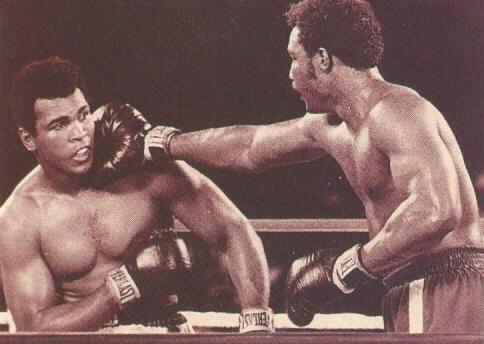
\includegraphics{images/ali.png}
	\footnote{\url{http://bit.ly/1OyIoEI}}
\end{frame}


\begin{frame}{Optimization of aversive reflexes}
	\begin{itemize}
		\item Avoid aversive stimuli with minimum necessary effort
		\item How we behave carries a cost: What we fail to prevent + preventing action itself
		\item The ideal actions are those that minimize the overall cost
	\end{itemize}
	[@Brandi2013]
\end{frame}


\begin{frame}{Nucleo-olivary inhibition (NOI)}
	\begin{columns}[T]
		\begin{column}[T]{5cm}
			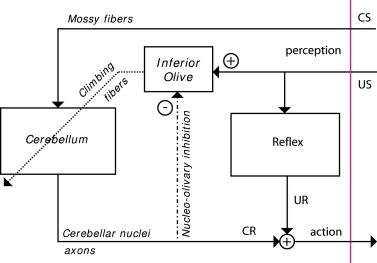
\includegraphics[]{images/noi.jpg}
		\end{column}
		\begin{column}[T]{5cm}
			\begin{itemize}
				\item Cost-optimization
				\item Error-based learning
				\item Acquired conditioned responses are extinguished once they become no longer necessary
				\item The gain of the NOI is what determines the amplitude of the response on adaptive reflexes
			\end{itemize}
		\end{column}
	\end{columns}
	[@Herreros2013b]
\end{frame}


\begin{frame}{NOI on eye-blink reflex}
	\begin{itemize}
		\item Perceiving an air-puff in the unprotected cornea has a cost
		\item Two types of costs
		\begin{itemize}
			\item Failing to avoid: error-based learning
			\item Avoiding when not necessary
		\end{itemize}
		\item Extinction of unnecessary conditioned responses
	\end{itemize}
	[@Herreros2013b]
\end{frame}


\begin{frame}{Vestibulo-ocular reflex (VOR)}
	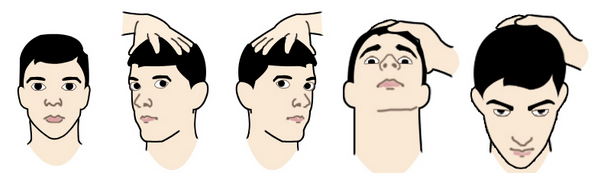
\includegraphics{images/vor.png}
	\footnote{\url{http://bit.ly/1Ox3Qd6}}
	This reflex functions to \textbf{stabilize images} on the retinas during \textbf{head movement} by producing \textbf{eye movements} in the direction opposite to head movement, thus preserving the image on the center of the visual field.
\end{frame}


\begin{frame}{Problem statement}
	\begin{quote}
		Computational models of the vestibulo-ocular reflex don't take into account the role of the nucleo-olivary inhibition
	\end{quote}
\end{frame}


\begin{frame}{Research question}
	\begin{quote}
		What's the role of the nucleo-olivary inhibition in the vestibulo-ocular reflex?
	\end{quote}
	\begin{block}{Fingerprints}
		\begin{itemize}
			\item NOI has a role in the eye-blink reflex
			\item There is extinction of the adaptive response in the absence of peripheral error
			\item VOR adaptation has a non-perfect performance, with a residual error proportional to the amount of cerebellar action required
		\end{itemize}
	[@Herreros2013b]
	\end{block}
\end{frame}


\begin{frame}{Hypothesis}
	\begin{quote}
		Adding nucleo-olivary inhibition on a detailed bottom-up state of the art vestibulo-ocular reflex computational model would offer a more
		parsimonious explanation of the experimental behavior of the reflex.
	\end{quote}
\end{frame}


\begin{frame}{Cerebellar cortex}
	\begin{columns}[T]
		\begin{column}[T]{5cm}
			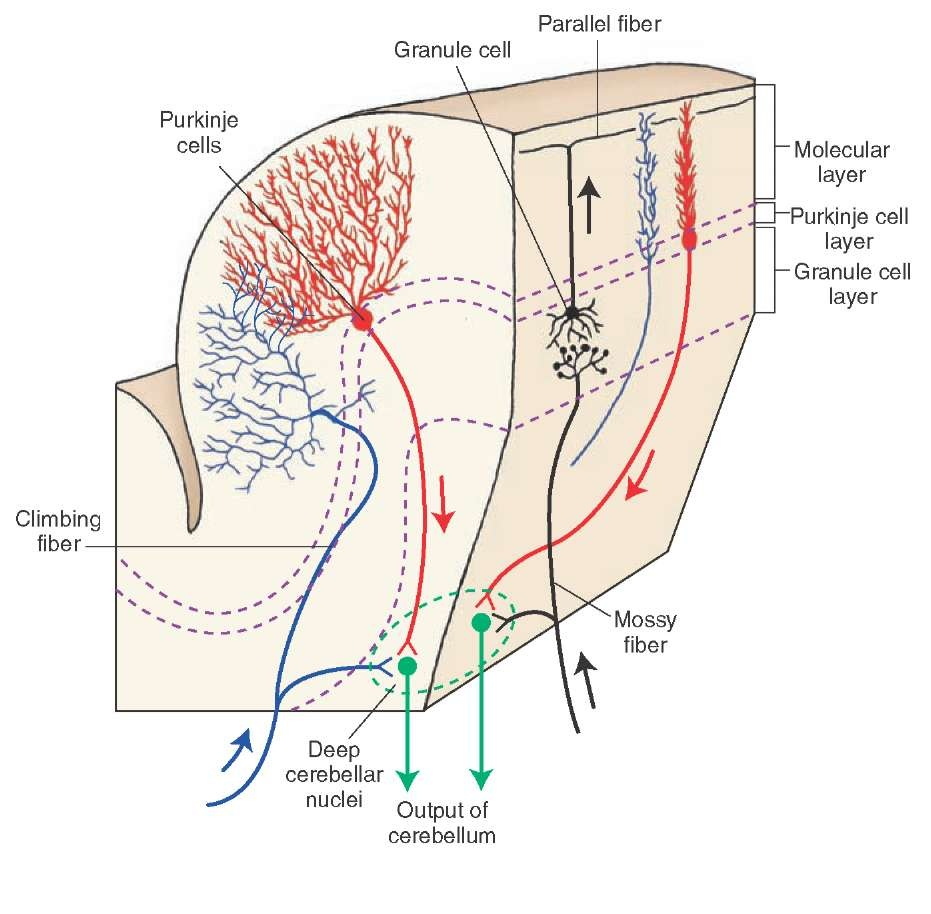
\includegraphics[height=3cm]{images/tmp15F112.jpg}
		\end{column}
		\begin{column}[T]{5cm}
			\begin{itemize}
				\item Uniform structure throughout the cerebellum
				\item Composed of repeated modules or microzones
				\item Same cell types and connectivity
				\item Functional units
				\item Different inputs, different targets
				\item Cerebellar algorithm
			\end{itemize}
		\end{column}
	\end{columns}
	\footnote{\url{http://bit.ly/1CioLvp}}
\end{frame}


\begin{frame}{Computational models of the VOR}
\end{frame}


\begin{frame}{A detailed bottom-up model}
	This computational model is made bottom-up from physiological and behavioral observations.
	\begin{itemize}
		\item Plasticity on the cerebellar cortex
		\item Plasticity on the brainstem
		\item Delayed error signal
		\item White noise on the signals
		\item Contribution of interneurons
	\end{itemize}
	[@Clopath2014]
\end{frame}


\begin{frame}{Wolff training protocol}
\end{frame}